\documentclass[twoside]{book}

% Packages required by doxygen
\usepackage{fixltx2e}
\usepackage{calc}
\usepackage{doxygen}
\usepackage[export]{adjustbox} % also loads graphicx
\usepackage{graphicx}
\usepackage[utf8]{inputenc}
\usepackage{makeidx}
\usepackage{multicol}
\usepackage{multirow}
\PassOptionsToPackage{warn}{textcomp}
\usepackage{textcomp}
\usepackage[nointegrals]{wasysym}
\usepackage[table]{xcolor}

% NLS support packages
\usepackage[T2A]{fontenc}
\usepackage[russian]{babel}

% Font selection
\usepackage[T1]{fontenc}
\usepackage[scaled=.90]{helvet}
\usepackage{courier}
\usepackage{amssymb}
\usepackage{sectsty}
\renewcommand{\familydefault}{\sfdefault}
\allsectionsfont{%
  \fontseries{bc}\selectfont%
  \color{darkgray}%
}
\renewcommand{\DoxyLabelFont}{%
  \fontseries{bc}\selectfont%
  \color{darkgray}%
}
\newcommand{\+}{\discretionary{\mbox{\scriptsize$\hookleftarrow$}}{}{}}

% Page & text layout
\usepackage{geometry}
\geometry{%
  a4paper,%
  top=2.5cm,%
  bottom=2.5cm,%
  left=2.5cm,%
  right=2.5cm%
}
\tolerance=750
\hfuzz=15pt
\hbadness=750
\setlength{\emergencystretch}{15pt}
\setlength{\parindent}{0cm}
\setlength{\parskip}{3ex plus 2ex minus 2ex}
\makeatletter
\renewcommand{\paragraph}{%
  \@startsection{paragraph}{4}{0ex}{-1.0ex}{1.0ex}{%
    \normalfont\normalsize\bfseries\SS@parafont%
  }%
}
\renewcommand{\subparagraph}{%
  \@startsection{subparagraph}{5}{0ex}{-1.0ex}{1.0ex}{%
    \normalfont\normalsize\bfseries\SS@subparafont%
  }%
}
\makeatother

% Headers & footers
\usepackage{fancyhdr}
\pagestyle{fancyplain}
\fancyhead[LE]{\fancyplain{}{\bfseries\thepage}}
\fancyhead[CE]{\fancyplain{}{}}
\fancyhead[RE]{\fancyplain{}{\bfseries\leftmark}}
\fancyhead[LO]{\fancyplain{}{\bfseries\rightmark}}
\fancyhead[CO]{\fancyplain{}{}}
\fancyhead[RO]{\fancyplain{}{\bfseries\thepage}}
\fancyfoot[LE]{\fancyplain{}{}}
\fancyfoot[CE]{\fancyplain{}{}}
\fancyfoot[RE]{\fancyplain{}{\bfseries\scriptsize Создано системой Doxygen }}
\fancyfoot[LO]{\fancyplain{}{\bfseries\scriptsize Создано системой Doxygen }}
\fancyfoot[CO]{\fancyplain{}{}}
\fancyfoot[RO]{\fancyplain{}{}}
\renewcommand{\footrulewidth}{0.4pt}
\renewcommand{\chaptermark}[1]{%
  \markboth{#1}{}%
}
\renewcommand{\sectionmark}[1]{%
  \markright{\thesection\ #1}%
}

% Indices & bibliography
\usepackage{natbib}
\usepackage[titles]{tocloft}
\setcounter{tocdepth}{3}
\setcounter{secnumdepth}{5}
\makeindex

% Packages requested by user
\usepackage{pscyr}

% Hyperlinks (required, but should be loaded last)
\usepackage{ifpdf}
\ifpdf
  \usepackage[pdftex,pagebackref=true]{hyperref}
\else
  \usepackage[ps2pdf,pagebackref=true]{hyperref}
\fi
\hypersetup{%
  colorlinks=true,%
  linkcolor=blue,%
  citecolor=blue,%
  unicode%
}

% Custom commands
\newcommand{\clearemptydoublepage}{%
  \newpage{\pagestyle{empty}\cleardoublepage}%
}

\usepackage{caption}
\captionsetup{labelsep=space,justification=centering,font={bf},singlelinecheck=off,skip=4pt,position=top}

%===== C O N T E N T S =====

\begin{document}

% Titlepage & ToC
\hypersetup{pageanchor=false,
             bookmarksnumbered=true,
             pdfencoding=unicode
            }
\pagenumbering{roman}
\begin{titlepage}
\vspace*{7cm}
\begin{center}%
{\Large Автоматизация конфигурирования сетевого оборудования Cisco }\\
\vspace*{1cm}
{\large Создано системой Doxygen 1.8.11}\\
\end{center}
\end{titlepage}
\clearemptydoublepage
\tableofcontents
\clearemptydoublepage
\pagenumbering{arabic}
\hypersetup{pageanchor=true}

%--- Begin generated contents ---
\chapter{Иерархический список классов}
\section{Иерархия классов}
Иерархия классов.\begin{DoxyCompactList}
\item \contentsline{section}{Interface\+Model}{\pageref{class_interface_model}}{}
\item Q\+Abstract\+Table\+Model\begin{DoxyCompactList}
\item \contentsline{section}{Interface\+Model\+List}{\pageref{class_interface_model_list}}{}
\end{DoxyCompactList}
\item \contentsline{section}{Q\+List$<$ T $>$}{\pageref{class_q_list}}{}
\item \contentsline{section}{Q\+List$<$ Interface\+Model $\ast$ $>$}{\pageref{class_q_list}}{}
\item Q\+Main\+Window\begin{DoxyCompactList}
\item \contentsline{section}{Main\+Window}{\pageref{class_main_window}}{}
\end{DoxyCompactList}
\item Q\+Object\begin{DoxyCompactList}
\item \contentsline{section}{Network\+Equipment\+Model}{\pageref{class_network_equipment_model}}{}
\end{DoxyCompactList}
\item Q\+Validator\begin{DoxyCompactList}
\item \contentsline{section}{Ipv4\+Validator}{\pageref{class_ipv4_validator}}{}
\item \contentsline{section}{Ipv6\+Validator}{\pageref{class_ipv6_validator}}{}
\item \contentsline{section}{Text\+Validator}{\pageref{class_text_validator}}{}
\item \contentsline{section}{Word\+Validator}{\pageref{class_word_validator}}{}
\end{DoxyCompactList}
\item Q\+Widget\begin{DoxyCompactList}
\item \contentsline{section}{Network\+Equipment\+Form}{\pageref{class_network_equipment_form}}{}
\end{DoxyCompactList}
\end{DoxyCompactList}

\chapter{Алфавитный указатель классов}
\section{Классы}
Классы с их кратким описанием.\begin{DoxyCompactList}
\item\contentsline{section}{\hyperlink{class_interface_model}{Interface\+Model} }{\pageref{class_interface_model}}{}
\item\contentsline{section}{\hyperlink{class_interface_model_list}{Interface\+Model\+List} }{\pageref{class_interface_model_list}}{}
\item\contentsline{section}{\hyperlink{class_ipv4_validator}{Ipv4\+Validator} }{\pageref{class_ipv4_validator}}{}
\item\contentsline{section}{\hyperlink{class_ipv6_validator}{Ipv6\+Validator} }{\pageref{class_ipv6_validator}}{}
\item\contentsline{section}{\hyperlink{class_main_window}{Main\+Window} }{\pageref{class_main_window}}{}
\item\contentsline{section}{\hyperlink{class_network_equipment_form}{Network\+Equipment\+Form} }{\pageref{class_network_equipment_form}}{}
\item\contentsline{section}{\hyperlink{class_network_equipment_model}{Network\+Equipment\+Model} \\*Модель сетевого оборудования }{\pageref{class_network_equipment_model}}{}
\item\contentsline{section}{\hyperlink{class_q_list}{Q\+List$<$ T $>$} }{\pageref{class_q_list}}{}
\item\contentsline{section}{\hyperlink{class_text_validator}{Text\+Validator} }{\pageref{class_text_validator}}{}
\item\contentsline{section}{\hyperlink{class_word_validator}{Word\+Validator} }{\pageref{class_word_validator}}{}
\end{DoxyCompactList}

\chapter{Классы}
\hypertarget{class_interface_model}{}\section{Класс Interface\+Model}
\label{class_interface_model}\index{Interface\+Model@{Interface\+Model}}
\subsection*{Открытые члены}
\begin{DoxyCompactItemize}
\item 
Interface\+Type {\bfseries type} ()\hypertarget{class_interface_model_ab9a3cf858cda42f7f21d86c701ed9baa}{}\label{class_interface_model_ab9a3cf858cda42f7f21d86c701ed9baa}

\item 
void {\bfseries set\+Type} (Interface\+Type type)\hypertarget{class_interface_model_a6d1e3a33e22e61dfbc860a23016b936e}{}\label{class_interface_model_a6d1e3a33e22e61dfbc860a23016b936e}

\item 
Q\+String {\bfseries number} ()\hypertarget{class_interface_model_ab7d36b21ece7aaeff0ad1399eaee6877}{}\label{class_interface_model_ab7d36b21ece7aaeff0ad1399eaee6877}

\item 
void {\bfseries set\+Number} (Q\+String number)\hypertarget{class_interface_model_a7bf6cec7997845df02b48a09c8edbb6d}{}\label{class_interface_model_a7bf6cec7997845df02b48a09c8edbb6d}

\item 
Q\+String {\bfseries description} ()\hypertarget{class_interface_model_a3d75ae4692a1b497a5677dda6592ee32}{}\label{class_interface_model_a3d75ae4692a1b497a5677dda6592ee32}

\item 
void {\bfseries set\+Description} (Q\+String description)\hypertarget{class_interface_model_a720fa2dcb0864bc64204e248314ac5a7}{}\label{class_interface_model_a720fa2dcb0864bc64204e248314ac5a7}

\item 
Duplex {\bfseries duplex} ()\hypertarget{class_interface_model_ae3ccb29aa96cf1d859091d5ebc213fde}{}\label{class_interface_model_ae3ccb29aa96cf1d859091d5ebc213fde}

\item 
void {\bfseries set\+Duplex} (Duplex duplex)\hypertarget{class_interface_model_a9f82d7f6f71fe196a55ed6bbc32a2809}{}\label{class_interface_model_a9f82d7f6f71fe196a55ed6bbc32a2809}

\item 
Q\+Host\+Address {\bfseries ipv4} ()\hypertarget{class_interface_model_a1601e72efd97a651dbc4541387afe47b}{}\label{class_interface_model_a1601e72efd97a651dbc4541387afe47b}

\item 
void {\bfseries set\+Ipv4} (Q\+Host\+Address ip)\hypertarget{class_interface_model_a0e4826c6024f3ea4a229df52809f8c17}{}\label{class_interface_model_a0e4826c6024f3ea4a229df52809f8c17}

\item 
Q\+Host\+Address {\bfseries ipv6} ()\hypertarget{class_interface_model_a4c5651b1ced869c27937443f073dd609}{}\label{class_interface_model_a4c5651b1ced869c27937443f073dd609}

\item 
void {\bfseries set\+Ipv6} (Q\+Host\+Address ip)\hypertarget{class_interface_model_af486a90f09c150d2e45a780b73145bb0}{}\label{class_interface_model_af486a90f09c150d2e45a780b73145bb0}

\end{DoxyCompactItemize}


Объявления и описания членов классов находятся в файлах\+:\begin{DoxyCompactItemize}
\item 
interfacemodel.\+h\item 
interfacemodel.\+cpp\end{DoxyCompactItemize}

\hypertarget{class_interface_model_list}{}\section{Класс Interface\+Model\+List}
\label{class_interface_model_list}\index{Interface\+Model\+List@{Interface\+Model\+List}}
Граф наследования\+:Interface\+Model\+List\+:\begin{figure}[H]
\begin{center}
\leavevmode
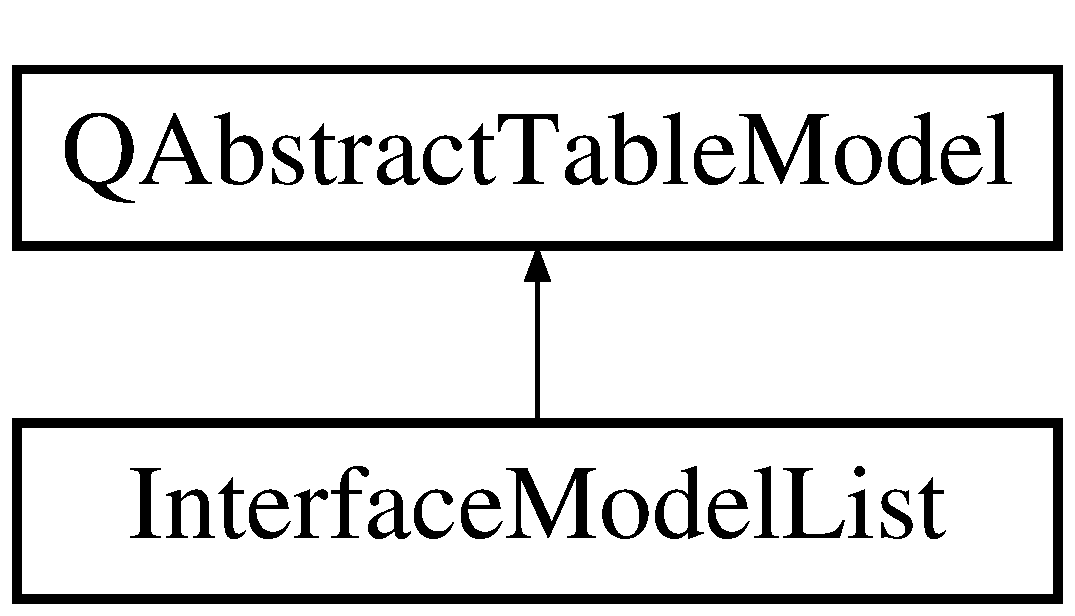
\includegraphics[height=2.000000cm]{class_interface_model_list}
\end{center}
\end{figure}
\subsection*{Открытые члены}
\begin{DoxyCompactItemize}
\item 
{\bfseries Interface\+Model\+List} (Q\+Object $\ast$parent)\hypertarget{class_interface_model_list_a926a7248c32335cb27669f0220b2a1b5}{}\label{class_interface_model_list_a926a7248c32335cb27669f0220b2a1b5}

\item 
int {\bfseries row\+Count} (const Q\+Model\+Index \&parent=Q\+Model\+Index()) const \hypertarget{class_interface_model_list_ad8846f668c2fbffdd8de7cb602e775d4}{}\label{class_interface_model_list_ad8846f668c2fbffdd8de7cb602e775d4}

\item 
int {\bfseries column\+Count} (const Q\+Model\+Index \&parent=Q\+Model\+Index()) const \hypertarget{class_interface_model_list_a590c92f0cca76b9838a1537bd5d34518}{}\label{class_interface_model_list_a590c92f0cca76b9838a1537bd5d34518}

\item 
Q\+Variant {\bfseries data} (const Q\+Model\+Index \&index, int role=Qt\+::\+Display\+Role) const \hypertarget{class_interface_model_list_a4c319165cc4c9ce42530ba40c5f6ae48}{}\label{class_interface_model_list_a4c319165cc4c9ce42530ba40c5f6ae48}

\item 
void {\bfseries set\+Interfaces} (\hyperlink{class_q_list}{Q\+List}$<$ \hyperlink{class_interface_model}{Interface\+Model} $\ast$ $>$ interfaces)\hypertarget{class_interface_model_list_a90c904fdb3e2c825d565e8acadab864e}{}\label{class_interface_model_list_a90c904fdb3e2c825d565e8acadab864e}

\end{DoxyCompactItemize}


Объявления и описания членов классов находятся в файлах\+:\begin{DoxyCompactItemize}
\item 
interfacemodel.\+h\item 
interfacemodel.\+cpp\end{DoxyCompactItemize}

\hypertarget{class_ipv4_validator}{}\section{Класс Ipv4\+Validator}
\label{class_ipv4_validator}\index{Ipv4\+Validator@{Ipv4\+Validator}}
Граф наследования\+:Ipv4\+Validator\+:\begin{figure}[H]
\begin{center}
\leavevmode
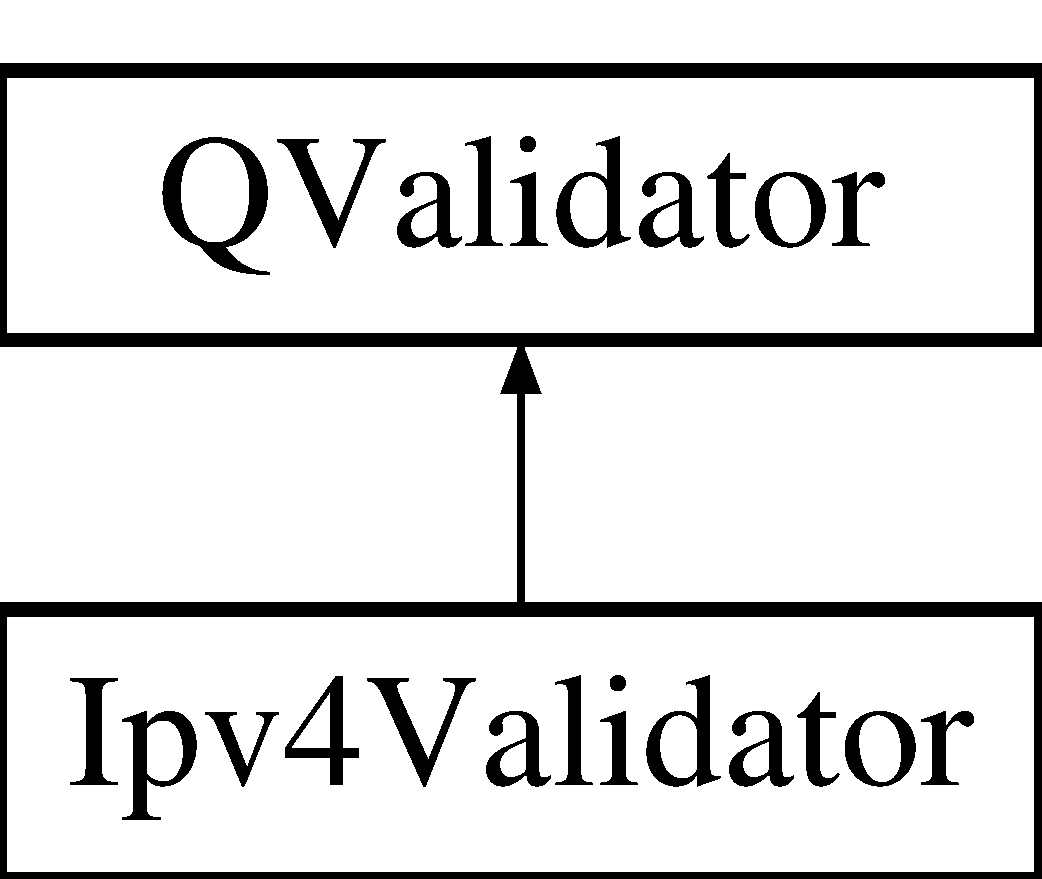
\includegraphics[height=2.000000cm]{class_ipv4_validator}
\end{center}
\end{figure}
\subsection*{Открытые члены}
\begin{DoxyCompactItemize}
\item 
\hyperlink{class_ipv4_validator_a5be0312dd5dfc0879eb9dc728a4ff577}{Ipv4\+Validator} (Q\+Object $\ast$parent=0)
\begin{DoxyCompactList}\small\item\em \hyperlink{class_ipv4_validator_a5be0312dd5dfc0879eb9dc728a4ff577}{Ipv4\+Validator\+::\+Ipv4\+Validator}. \end{DoxyCompactList}\item 
State \hyperlink{class_ipv4_validator_a6e5095efeaf75e97c1842b8c42db7c03}{validate} (Q\+String \&, int \&) const 
\begin{DoxyCompactList}\small\item\em \hyperlink{class_ipv4_validator_a6e5095efeaf75e97c1842b8c42db7c03}{Ipv4\+Validator\+::validate}. \end{DoxyCompactList}\end{DoxyCompactItemize}


\subsection{Конструктор(ы)}
\index{Ipv4\+Validator@{Ipv4\+Validator}!Ipv4\+Validator@{Ipv4\+Validator}}
\index{Ipv4\+Validator@{Ipv4\+Validator}!Ipv4\+Validator@{Ipv4\+Validator}}
\subsubsection[{\texorpdfstring{Ipv4\+Validator(\+Q\+Object $\ast$parent=0)}{Ipv4Validator(QObject *parent=0)}}]{\setlength{\rightskip}{0pt plus 5cm}Ipv4\+Validator\+::\+Ipv4\+Validator (
\begin{DoxyParamCaption}
\item[{Q\+Object $\ast$}]{parent = {\ttfamily 0}}
\end{DoxyParamCaption}
)}\hypertarget{class_ipv4_validator_a5be0312dd5dfc0879eb9dc728a4ff577}{}\label{class_ipv4_validator_a5be0312dd5dfc0879eb9dc728a4ff577}


\hyperlink{class_ipv4_validator_a5be0312dd5dfc0879eb9dc728a4ff577}{Ipv4\+Validator\+::\+Ipv4\+Validator}. 


\begin{DoxyParams}{Аргументы}
{\em parent} & \\
\hline
\end{DoxyParams}


\subsection{Методы}
\index{Ipv4\+Validator@{Ipv4\+Validator}!validate@{validate}}
\index{validate@{validate}!Ipv4\+Validator@{Ipv4\+Validator}}
\subsubsection[{\texorpdfstring{validate(\+Q\+String \&, int \&) const }{validate(QString &, int &) const }}]{\setlength{\rightskip}{0pt plus 5cm}Q\+Validator\+::\+State Ipv4\+Validator\+::validate (
\begin{DoxyParamCaption}
\item[{Q\+String \&}]{text, }
\item[{int \&}]{pos}
\end{DoxyParamCaption}
) const}\hypertarget{class_ipv4_validator_a6e5095efeaf75e97c1842b8c42db7c03}{}\label{class_ipv4_validator_a6e5095efeaf75e97c1842b8c42db7c03}


\hyperlink{class_ipv4_validator_a6e5095efeaf75e97c1842b8c42db7c03}{Ipv4\+Validator\+::validate}. 


\begin{DoxyParams}{Аргументы}
{\em text} & \\
\hline
{\em pos} & \\
\hline
\end{DoxyParams}
\begin{DoxyReturn}{Возвращает}

\end{DoxyReturn}


Объявления и описания членов классов находятся в файлах\+:\begin{DoxyCompactItemize}
\item 
customvalidator.\+h\item 
customvalidator.\+cpp\end{DoxyCompactItemize}

\hypertarget{class_ipv6_validator}{}\section{Класс Ipv6\+Validator}
\label{class_ipv6_validator}\index{Ipv6\+Validator@{Ipv6\+Validator}}
Граф наследования\+:Ipv6\+Validator\+:\begin{figure}[H]
\begin{center}
\leavevmode
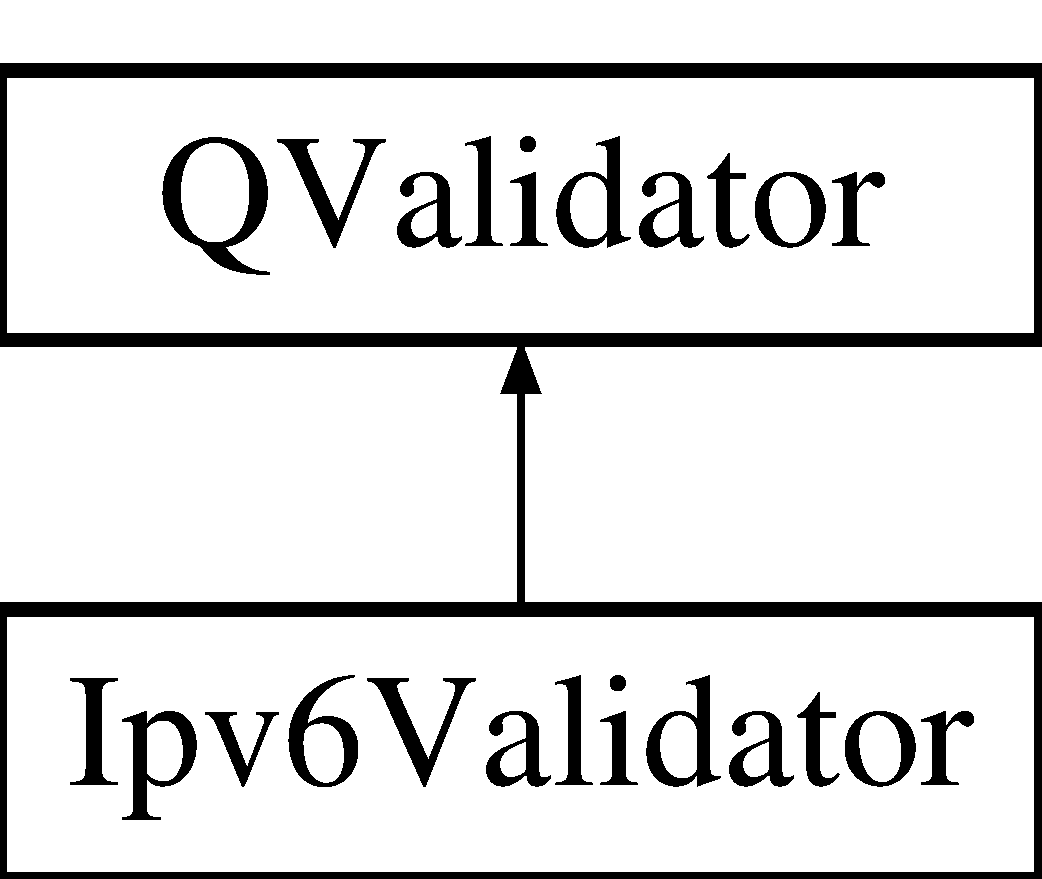
\includegraphics[height=2.000000cm]{class_ipv6_validator}
\end{center}
\end{figure}
\subsection*{Открытые члены}
\begin{DoxyCompactItemize}
\item 
\hyperlink{class_ipv6_validator_a2caeac54ee2995a6ac4b7716a52314f3}{Ipv6\+Validator} (Q\+Object $\ast$parent=0)
\begin{DoxyCompactList}\small\item\em \hyperlink{class_ipv6_validator_a2caeac54ee2995a6ac4b7716a52314f3}{Ipv6\+Validator\+::\+Ipv6\+Validator}. \end{DoxyCompactList}\item 
State \hyperlink{class_ipv6_validator_a847681eac42c4b238a3b3e8c8c5d18c2}{validate} (Q\+String \&, int \&) const 
\begin{DoxyCompactList}\small\item\em \hyperlink{class_ipv6_validator_a847681eac42c4b238a3b3e8c8c5d18c2}{Ipv6\+Validator\+::validate}. \end{DoxyCompactList}\end{DoxyCompactItemize}


\subsection{Конструктор(ы)}
\index{Ipv6\+Validator@{Ipv6\+Validator}!Ipv6\+Validator@{Ipv6\+Validator}}
\index{Ipv6\+Validator@{Ipv6\+Validator}!Ipv6\+Validator@{Ipv6\+Validator}}
\subsubsection[{\texorpdfstring{Ipv6\+Validator(\+Q\+Object $\ast$parent=0)}{Ipv6Validator(QObject *parent=0)}}]{\setlength{\rightskip}{0pt plus 5cm}Ipv6\+Validator\+::\+Ipv6\+Validator (
\begin{DoxyParamCaption}
\item[{Q\+Object $\ast$}]{parent = {\ttfamily 0}}
\end{DoxyParamCaption}
)}\hypertarget{class_ipv6_validator_a2caeac54ee2995a6ac4b7716a52314f3}{}\label{class_ipv6_validator_a2caeac54ee2995a6ac4b7716a52314f3}


\hyperlink{class_ipv6_validator_a2caeac54ee2995a6ac4b7716a52314f3}{Ipv6\+Validator\+::\+Ipv6\+Validator}. 


\begin{DoxyParams}{Аргументы}
{\em parent} & \\
\hline
\end{DoxyParams}


\subsection{Методы}
\index{Ipv6\+Validator@{Ipv6\+Validator}!validate@{validate}}
\index{validate@{validate}!Ipv6\+Validator@{Ipv6\+Validator}}
\subsubsection[{\texorpdfstring{validate(\+Q\+String \&, int \&) const }{validate(QString &, int &) const }}]{\setlength{\rightskip}{0pt plus 5cm}Q\+Validator\+::\+State Ipv6\+Validator\+::validate (
\begin{DoxyParamCaption}
\item[{Q\+String \&}]{text, }
\item[{int \&}]{pos}
\end{DoxyParamCaption}
) const}\hypertarget{class_ipv6_validator_a847681eac42c4b238a3b3e8c8c5d18c2}{}\label{class_ipv6_validator_a847681eac42c4b238a3b3e8c8c5d18c2}


\hyperlink{class_ipv6_validator_a847681eac42c4b238a3b3e8c8c5d18c2}{Ipv6\+Validator\+::validate}. 


\begin{DoxyParams}{Аргументы}
{\em text} & \\
\hline
{\em pos} & \\
\hline
\end{DoxyParams}
\begin{DoxyReturn}{Возвращает}

\end{DoxyReturn}


Объявления и описания членов классов находятся в файлах\+:\begin{DoxyCompactItemize}
\item 
customvalidator.\+h\item 
customvalidator.\+cpp\end{DoxyCompactItemize}

\hypertarget{class_main_window}{}\section{Класс Main\+Window}
\label{class_main_window}\index{Main\+Window@{Main\+Window}}
Граф наследования\+:Main\+Window\+:\begin{figure}[H]
\begin{center}
\leavevmode
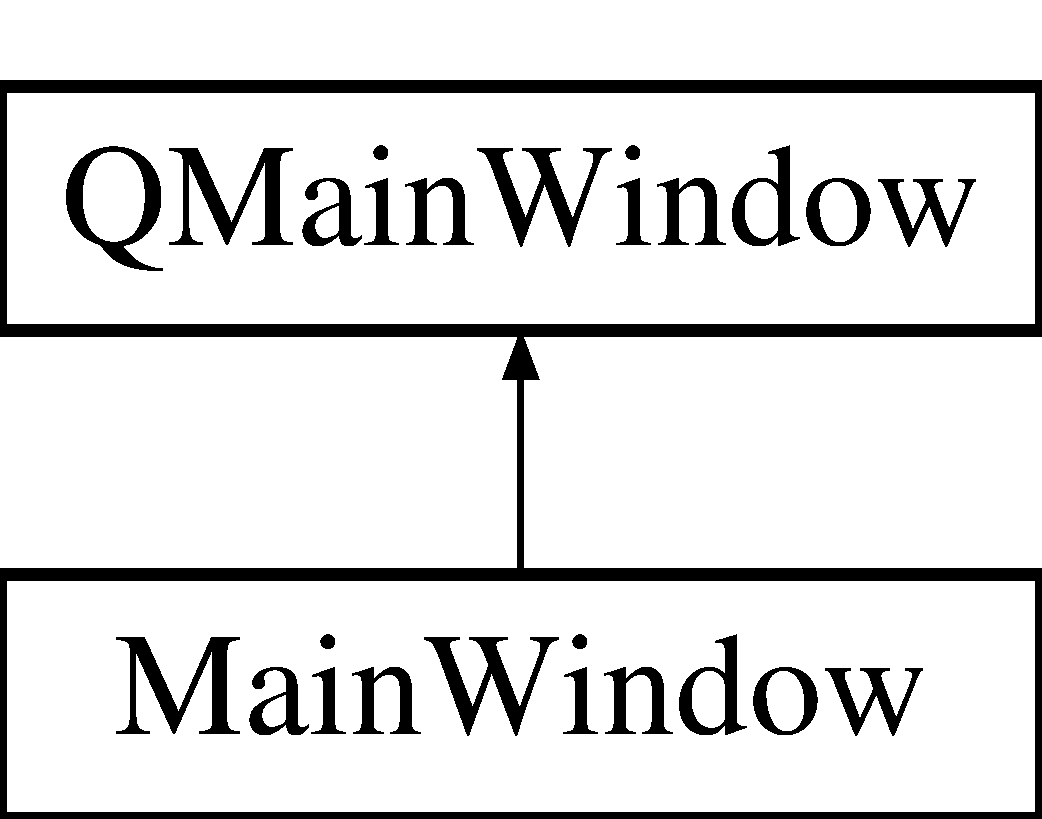
\includegraphics[height=2.000000cm]{class_main_window}
\end{center}
\end{figure}
\subsection*{Открытые члены}
\begin{DoxyCompactItemize}
\item 
{\bfseries Main\+Window} (Q\+Widget $\ast$parent=0)\hypertarget{class_main_window_a8b244be8b7b7db1b08de2a2acb9409db}{}\label{class_main_window_a8b244be8b7b7db1b08de2a2acb9409db}

\end{DoxyCompactItemize}


Объявления и описания членов классов находятся в файлах\+:\begin{DoxyCompactItemize}
\item 
mainwindow.\+h\item 
mainwindow.\+cpp\end{DoxyCompactItemize}

\hypertarget{class_network_equipment_form}{}\section{Класс Network\+Equipment\+Form}
\label{class_network_equipment_form}\index{Network\+Equipment\+Form@{Network\+Equipment\+Form}}
Граф наследования\+:Network\+Equipment\+Form\+:\begin{figure}[H]
\begin{center}
\leavevmode
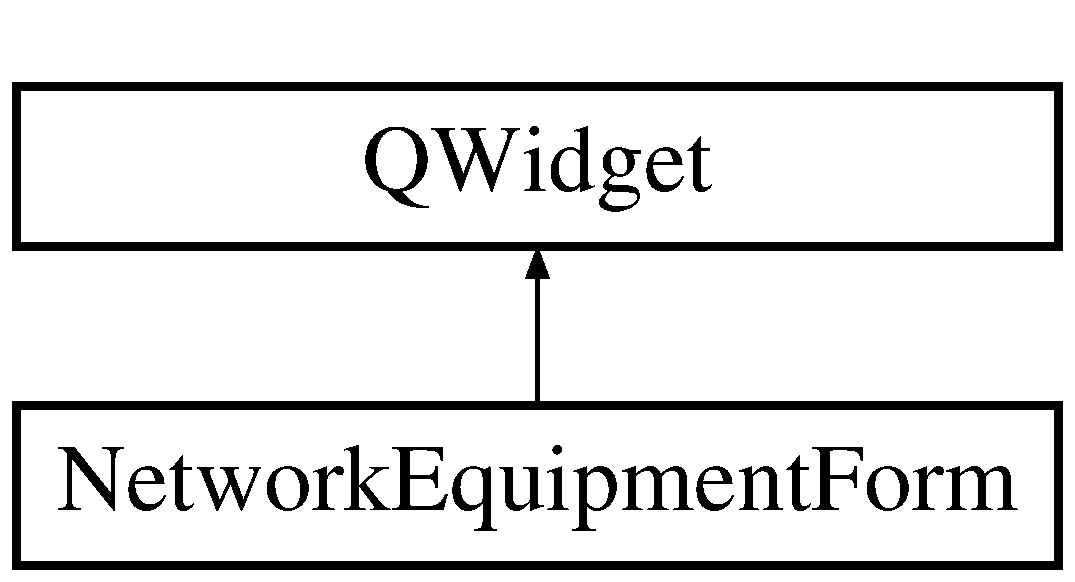
\includegraphics[height=2.000000cm]{class_network_equipment_form}
\end{center}
\end{figure}
\subsection*{Открытые слоты}
\begin{DoxyCompactItemize}
\item 
virtual void {\bfseries set\+Need\+Hostname} (bool need\+Hostname)\hypertarget{class_network_equipment_form_aa4f27acc75a23ad6217c73d1993d0376}{}\label{class_network_equipment_form_aa4f27acc75a23ad6217c73d1993d0376}

\item 
virtual void {\bfseries set\+Hostname} (Q\+String hostname)\hypertarget{class_network_equipment_form_a1752541512a46670f6febf6b72cf5982}{}\label{class_network_equipment_form_a1752541512a46670f6febf6b72cf5982}

\item 
virtual void {\bfseries set\+Password\+Encryption} (bool password\+Encryption)\hypertarget{class_network_equipment_form_a0d9eb5989eb412d6280932312e9b20ac}{}\label{class_network_equipment_form_a0d9eb5989eb412d6280932312e9b20ac}

\item 
virtual void {\bfseries set\+Need\+Banner\+Motd} (bool need\+Banner\+Motd)\hypertarget{class_network_equipment_form_a2afda0d1433c5d628a64fdd8257c3eea}{}\label{class_network_equipment_form_a2afda0d1433c5d628a64fdd8257c3eea}

\item 
virtual void {\bfseries set\+Banner\+Motd} (Q\+String banner\+Motd)\hypertarget{class_network_equipment_form_a79f90ee6080427b546440919fda03a63}{}\label{class_network_equipment_form_a79f90ee6080427b546440919fda03a63}

\item 
virtual void {\bfseries set\+Logging\+Synchronous} (bool logging\+Synchronous)\hypertarget{class_network_equipment_form_a648fbcdd8f69b64eab22da3ebb1f962f}{}\label{class_network_equipment_form_a648fbcdd8f69b64eab22da3ebb1f962f}

\item 
virtual void {\bfseries set\+Need\+Password\+Console} (bool need\+Password\+Console)\hypertarget{class_network_equipment_form_a47fbe2df13e3571ee14f74b40e0ee85c}{}\label{class_network_equipment_form_a47fbe2df13e3571ee14f74b40e0ee85c}

\item 
virtual void {\bfseries set\+Password\+Console} (Q\+String password)\hypertarget{class_network_equipment_form_a433f72d8df210acf7a77fcb96da9cd1b}{}\label{class_network_equipment_form_a433f72d8df210acf7a77fcb96da9cd1b}

\item 
virtual void {\bfseries set\+Need\+Password\+Vty} (bool need\+Password\+Vty)\hypertarget{class_network_equipment_form_a4c0fe8aa82ac42bd34f8f44f3f42e966}{}\label{class_network_equipment_form_a4c0fe8aa82ac42bd34f8f44f3f42e966}

\item 
virtual void {\bfseries set\+Password\+Vty} (Q\+String password)\hypertarget{class_network_equipment_form_a4a33264c3f13fc8795d3fce4d4a451cf}{}\label{class_network_equipment_form_a4a33264c3f13fc8795d3fce4d4a451cf}

\end{DoxyCompactItemize}
\subsection*{Открытые члены}
\begin{DoxyCompactItemize}
\item 
{\bfseries Network\+Equipment\+Form} (Q\+Widget $\ast$parent=0)\hypertarget{class_network_equipment_form_a1ee2a5fc8df7255d2887ff9a898c1139}{}\label{class_network_equipment_form_a1ee2a5fc8df7255d2887ff9a898c1139}

\item 
void {\bfseries set\+Model} (\hyperlink{class_network_equipment_model}{Network\+Equipment\+Model} $\ast$model)\hypertarget{class_network_equipment_form_a36fc9eb8d7f2a5ff79084661709a9936}{}\label{class_network_equipment_form_a36fc9eb8d7f2a5ff79084661709a9936}

\end{DoxyCompactItemize}


\subsection{Подробное описание}
Представление (View) в триаде M\+VP сетевого оборудования 

Объявления и описания членов классов находятся в файлах\+:\begin{DoxyCompactItemize}
\item 
networkequipmentform.\+h\item 
networkequipmentform.\+cpp\end{DoxyCompactItemize}

\hypertarget{class_network_equipment_model}{}\section{Класс Network\+Equipment\+Model}
\label{class_network_equipment_model}\index{Network\+Equipment\+Model@{Network\+Equipment\+Model}}


Модель сетевого оборудования  


Граф наследования\+:Network\+Equipment\+Model\+:\begin{figure}[H]
\begin{center}
\leavevmode
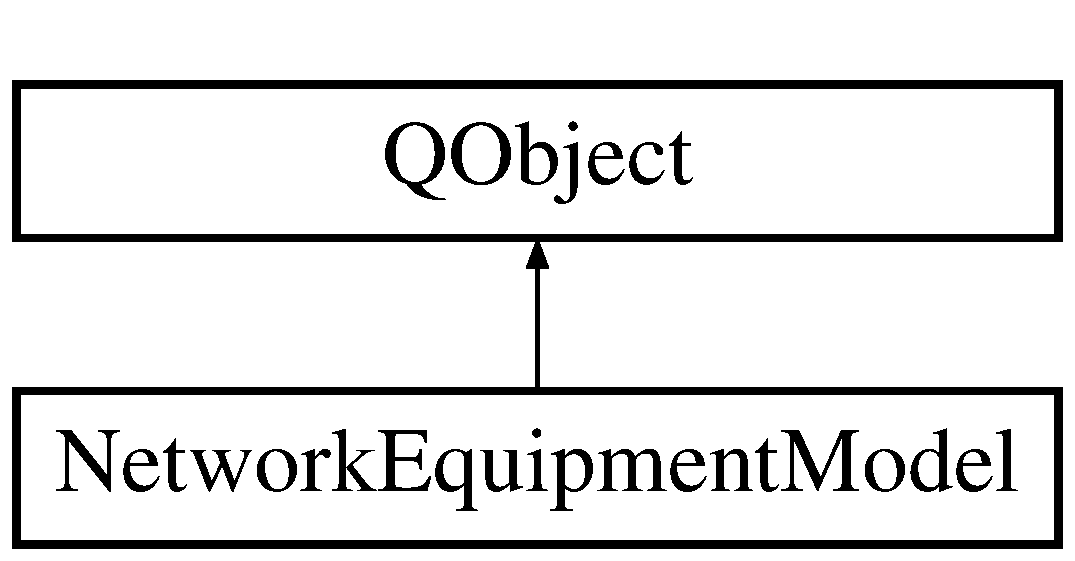
\includegraphics[height=2.000000cm]{class_network_equipment_model}
\end{center}
\end{figure}
\subsection*{Открытые слоты}
\begin{DoxyCompactItemize}
\item 
virtual void \hyperlink{class_network_equipment_model_a952a89f03887ab83ed42d404aad7acf4}{set\+Need\+Hostname} (bool \hyperlink{class_network_equipment_model_a67cb5cf3284a19a1a0d6a7b22fa2a91e}{need\+Hostname})
\begin{DoxyCompactList}\small\item\em Оболочка для установления необходимости называть оборудование \end{DoxyCompactList}\item 
virtual void \hyperlink{class_network_equipment_model_a844d05c49e462ea50dbf07b73597f65c}{set\+Hostname} (Q\+String \hyperlink{class_network_equipment_model_a59f5581ce5f16229235bc9ace24e11d6}{hostname})
\begin{DoxyCompactList}\small\item\em Оболочка для установки нового названия оборудования \end{DoxyCompactList}\item 
virtual void \hyperlink{class_network_equipment_model_a0303cb675bc0d42bff6b90d6e7b8bbb1}{set\+Password\+Encryption} (bool \hyperlink{class_network_equipment_model_a46900023e99e2791d5e0ff85204f25fb}{password\+Encryption})
\begin{DoxyCompactList}\small\item\em Оболочка для изменения необходимости скрывать пароли \end{DoxyCompactList}\item 
virtual void \hyperlink{class_network_equipment_model_a45955890b14b8dbd4f76df92cff2a82e}{set\+Need\+Banner\+Motd} (bool \hyperlink{class_network_equipment_model_ab20b1087ae50a8546bdabfa598e8c647}{need\+Banner\+Motd})
\begin{DoxyCompactList}\small\item\em Оболочка для установление необходимости указывать приветственное сообщение \end{DoxyCompactList}\item 
virtual void \hyperlink{class_network_equipment_model_a73bfb9a80a611f8925e23b4e68c95821}{set\+Banner\+Motd} (Q\+String \hyperlink{class_network_equipment_model_a9256503fdb609788939777565574ae7c}{banner\+Motd})
\begin{DoxyCompactList}\small\item\em Оболочка для изменения текущего текста приветствия \end{DoxyCompactList}\item 
virtual void \hyperlink{class_network_equipment_model_abe5f1892f0ca1bf727b8ceaf7baac189}{set\+Logging\+Synchronous} (bool \hyperlink{class_network_equipment_model_a7321ba74141fd1bc694a6607363625ae}{logging\+Synchronous})
\begin{DoxyCompactList}\small\item\em Оболочка для изменения запрета вывода каких-\/либо консольных сообщений при вводе команд в консольном режиме \end{DoxyCompactList}\item 
virtual void \hyperlink{class_network_equipment_model_afcdfd40284207e699e956dd3877a96c2}{set\+Need\+Password\+Console} (bool \hyperlink{class_network_equipment_model_ada70138a6ca4a8ad1bd07fa48998c9d8}{need\+Password\+Console})
\begin{DoxyCompactList}\small\item\em Оболочка для изменения необходимости ввода пароля при консольном подключении \end{DoxyCompactList}\item 
virtual void \hyperlink{class_network_equipment_model_aabfab95bca2f8b6b8d034662474e8dde}{set\+Password\+Console} (Q\+String password)
\begin{DoxyCompactList}\small\item\em Оболочка для изменения пароля при консольном подключении \end{DoxyCompactList}\item 
virtual void \hyperlink{class_network_equipment_model_a1d554674ebbe923251c73edb4832a470}{set\+Need\+Password\+Vty} (bool \hyperlink{class_network_equipment_model_aba3aec560271bbf72ee93fdf5e4c3a2e}{need\+Password\+Vty})
\begin{DoxyCompactList}\small\item\em Оболочка для изменения необходимости ввода пароля при терминальном подключении \end{DoxyCompactList}\item 
virtual void \hyperlink{class_network_equipment_model_ac6b735b52e9d5abef230bf6f0b475ab5}{set\+Password\+Vty} (Q\+String password)
\begin{DoxyCompactList}\small\item\em Оболочка для изменения пароля при терминальном подключении \end{DoxyCompactList}\end{DoxyCompactItemize}
\subsection*{Сигналы}
\begin{DoxyCompactItemize}
\item 
virtual void {\bfseries need\+Hostname\+Changed} (bool \hyperlink{class_network_equipment_model_a67cb5cf3284a19a1a0d6a7b22fa2a91e}{need\+Hostname})\hypertarget{class_network_equipment_model_a8c4c355442953dd22990b55eff5d1c87}{}\label{class_network_equipment_model_a8c4c355442953dd22990b55eff5d1c87}

\item 
virtual void {\bfseries hostname\+Changed} (Q\+String \hyperlink{class_network_equipment_model_a59f5581ce5f16229235bc9ace24e11d6}{hostname})\hypertarget{class_network_equipment_model_a022d6ce226b046705de3a2c1fd430e33}{}\label{class_network_equipment_model_a022d6ce226b046705de3a2c1fd430e33}

\item 
virtual void {\bfseries password\+Encryption\+Changed} (bool \hyperlink{class_network_equipment_model_a46900023e99e2791d5e0ff85204f25fb}{password\+Encryption})\hypertarget{class_network_equipment_model_ab8312ba3ebe2b6d3af20ebdafd90ec17}{}\label{class_network_equipment_model_ab8312ba3ebe2b6d3af20ebdafd90ec17}

\item 
virtual void {\bfseries need\+Banner\+Motd\+Changed} (bool \hyperlink{class_network_equipment_model_ab20b1087ae50a8546bdabfa598e8c647}{need\+Banner\+Motd})\hypertarget{class_network_equipment_model_ae4c88d5f5818022382a52b06e8d2fe73}{}\label{class_network_equipment_model_ae4c88d5f5818022382a52b06e8d2fe73}

\item 
virtual void {\bfseries banner\+Motd\+Changed} (Q\+String \hyperlink{class_network_equipment_model_a9256503fdb609788939777565574ae7c}{banner\+Motd})\hypertarget{class_network_equipment_model_a58ccbc2eadc43659e365316ad617ea18}{}\label{class_network_equipment_model_a58ccbc2eadc43659e365316ad617ea18}

\item 
virtual void {\bfseries logging\+Synchronous\+Changed} (bool \hyperlink{class_network_equipment_model_a7321ba74141fd1bc694a6607363625ae}{logging\+Synchronous})\hypertarget{class_network_equipment_model_a2f68757692a19aa6ead965f5d9850dbd}{}\label{class_network_equipment_model_a2f68757692a19aa6ead965f5d9850dbd}

\item 
virtual void {\bfseries need\+Password\+Console\+Changed} (bool \hyperlink{class_network_equipment_model_ada70138a6ca4a8ad1bd07fa48998c9d8}{need\+Password\+Console})\hypertarget{class_network_equipment_model_a1f0f610dad382795f3c18e01090bda98}{}\label{class_network_equipment_model_a1f0f610dad382795f3c18e01090bda98}

\item 
virtual void {\bfseries password\+Console\+Changed} (Q\+String password)\hypertarget{class_network_equipment_model_afcb0ebd93488fb50551e5464e3e7f307}{}\label{class_network_equipment_model_afcb0ebd93488fb50551e5464e3e7f307}

\item 
virtual void {\bfseries need\+Password\+Vty\+Changed} (bool \hyperlink{class_network_equipment_model_aba3aec560271bbf72ee93fdf5e4c3a2e}{need\+Password\+Vty})\hypertarget{class_network_equipment_model_a6a4774e0986ef76f12ca448b7c9933ad}{}\label{class_network_equipment_model_a6a4774e0986ef76f12ca448b7c9933ad}

\item 
virtual void {\bfseries password\+Vty\+Changed} (Q\+String password)\hypertarget{class_network_equipment_model_a5596328a92c1af7230b4efc793f6762d}{}\label{class_network_equipment_model_a5596328a92c1af7230b4efc793f6762d}

\end{DoxyCompactItemize}
\subsection*{Открытые члены}
\begin{DoxyCompactItemize}
\item 
{\bfseries Network\+Equipment\+Model} (Q\+Object $\ast$parent=0)\hypertarget{class_network_equipment_model_a757c88ce2d675d041d3539200f9f0a46}{}\label{class_network_equipment_model_a757c88ce2d675d041d3539200f9f0a46}

\item 
virtual bool \hyperlink{class_network_equipment_model_a67cb5cf3284a19a1a0d6a7b22fa2a91e}{need\+Hostname} ()
\begin{DoxyCompactList}\small\item\em Оболочка для получения необходимости называть оборудование \end{DoxyCompactList}\item 
virtual Q\+String \hyperlink{class_network_equipment_model_a59f5581ce5f16229235bc9ace24e11d6}{hostname} ()
\begin{DoxyCompactList}\small\item\em Оболочка для получения текущего названия оборудования \end{DoxyCompactList}\item 
virtual bool \hyperlink{class_network_equipment_model_a46900023e99e2791d5e0ff85204f25fb}{password\+Encryption} ()
\begin{DoxyCompactList}\small\item\em Оболочка для получения сведений о необходимости скрывать пароли \end{DoxyCompactList}\item 
virtual bool \hyperlink{class_network_equipment_model_ab20b1087ae50a8546bdabfa598e8c647}{need\+Banner\+Motd} ()
\begin{DoxyCompactList}\small\item\em Оболочка для получения необходимости указывать приветственное сообщение \end{DoxyCompactList}\item 
virtual Q\+String \hyperlink{class_network_equipment_model_a9256503fdb609788939777565574ae7c}{banner\+Motd} ()
\begin{DoxyCompactList}\small\item\em Оболочка для получения текущего текста приветствия \end{DoxyCompactList}\item 
virtual bool \hyperlink{class_network_equipment_model_a7321ba74141fd1bc694a6607363625ae}{logging\+Synchronous} ()
\begin{DoxyCompactList}\small\item\em Оболочка для получения сведений о запрете вывода каких-\/либо консольных сообщений при вводе команд в консольном режиме \end{DoxyCompactList}\item 
virtual bool \hyperlink{class_network_equipment_model_ada70138a6ca4a8ad1bd07fa48998c9d8}{need\+Password\+Console} ()
\begin{DoxyCompactList}\small\item\em Оболочка для получения сведений о необходимости ввода пароля при консольном подключении \end{DoxyCompactList}\item 
virtual Q\+String \hyperlink{class_network_equipment_model_a34400a7581340c475357034e3b183e5c}{password\+Console} ()
\begin{DoxyCompactList}\small\item\em Оболочка для получения пароля при консольном подключении \end{DoxyCompactList}\item 
virtual bool \hyperlink{class_network_equipment_model_aba3aec560271bbf72ee93fdf5e4c3a2e}{need\+Password\+Vty} ()
\begin{DoxyCompactList}\small\item\em Оболочка для изменения необходимости ввода пароля при терминальном подключении \end{DoxyCompactList}\item 
virtual Q\+String \hyperlink{class_network_equipment_model_a066e6c334dcf83f5f2646be4f8f19299}{password\+Vty} ()
\begin{DoxyCompactList}\small\item\em Оболочка для получения пароля при терминальном подключении \end{DoxyCompactList}\end{DoxyCompactItemize}


\subsection{Подробное описание}
Модель сетевого оборудования 

\subsection{Методы}
\index{Network\+Equipment\+Model@{Network\+Equipment\+Model}!banner\+Motd@{banner\+Motd}}
\index{banner\+Motd@{banner\+Motd}!Network\+Equipment\+Model@{Network\+Equipment\+Model}}
\subsubsection[{\texorpdfstring{banner\+Motd()}{bannerMotd()}}]{\setlength{\rightskip}{0pt plus 5cm}Q\+String Network\+Equipment\+Model\+::banner\+Motd (
\begin{DoxyParamCaption}
{}
\end{DoxyParamCaption}
)\hspace{0.3cm}{\ttfamily [virtual]}}\hypertarget{class_network_equipment_model_a9256503fdb609788939777565574ae7c}{}\label{class_network_equipment_model_a9256503fdb609788939777565574ae7c}


Оболочка для получения текущего текста приветствия 

\begin{DoxyReturn}{Возвращает}
текущий текст приветствия 
\end{DoxyReturn}
\index{Network\+Equipment\+Model@{Network\+Equipment\+Model}!hostname@{hostname}}
\index{hostname@{hostname}!Network\+Equipment\+Model@{Network\+Equipment\+Model}}
\subsubsection[{\texorpdfstring{hostname()}{hostname()}}]{\setlength{\rightskip}{0pt plus 5cm}Q\+String Network\+Equipment\+Model\+::hostname (
\begin{DoxyParamCaption}
{}
\end{DoxyParamCaption}
)\hspace{0.3cm}{\ttfamily [virtual]}}\hypertarget{class_network_equipment_model_a59f5581ce5f16229235bc9ace24e11d6}{}\label{class_network_equipment_model_a59f5581ce5f16229235bc9ace24e11d6}


Оболочка для получения текущего названия оборудования 

\begin{DoxyReturn}{Возвращает}
название оборудования 
\end{DoxyReturn}
\index{Network\+Equipment\+Model@{Network\+Equipment\+Model}!logging\+Synchronous@{logging\+Synchronous}}
\index{logging\+Synchronous@{logging\+Synchronous}!Network\+Equipment\+Model@{Network\+Equipment\+Model}}
\subsubsection[{\texorpdfstring{logging\+Synchronous()}{loggingSynchronous()}}]{\setlength{\rightskip}{0pt plus 5cm}bool Network\+Equipment\+Model\+::logging\+Synchronous (
\begin{DoxyParamCaption}
{}
\end{DoxyParamCaption}
)\hspace{0.3cm}{\ttfamily [virtual]}}\hypertarget{class_network_equipment_model_a7321ba74141fd1bc694a6607363625ae}{}\label{class_network_equipment_model_a7321ba74141fd1bc694a6607363625ae}


Оболочка для получения сведений о запрете вывода каких-\/либо консольных сообщений при вводе команд в консольном режиме 

\begin{DoxyReturn}{Возвращает}
сведения о запрете вывода каких-\/либо консольных сообщений при вводе команд в консольном режиме 
\end{DoxyReturn}
\index{Network\+Equipment\+Model@{Network\+Equipment\+Model}!need\+Banner\+Motd@{need\+Banner\+Motd}}
\index{need\+Banner\+Motd@{need\+Banner\+Motd}!Network\+Equipment\+Model@{Network\+Equipment\+Model}}
\subsubsection[{\texorpdfstring{need\+Banner\+Motd()}{needBannerMotd()}}]{\setlength{\rightskip}{0pt plus 5cm}bool Network\+Equipment\+Model\+::need\+Banner\+Motd (
\begin{DoxyParamCaption}
{}
\end{DoxyParamCaption}
)\hspace{0.3cm}{\ttfamily [virtual]}}\hypertarget{class_network_equipment_model_ab20b1087ae50a8546bdabfa598e8c647}{}\label{class_network_equipment_model_ab20b1087ae50a8546bdabfa598e8c647}


Оболочка для получения необходимости указывать приветственное сообщение 

\begin{DoxyReturn}{Возвращает}
необходимость указывать приветственное сообщение 
\end{DoxyReturn}
\index{Network\+Equipment\+Model@{Network\+Equipment\+Model}!need\+Hostname@{need\+Hostname}}
\index{need\+Hostname@{need\+Hostname}!Network\+Equipment\+Model@{Network\+Equipment\+Model}}
\subsubsection[{\texorpdfstring{need\+Hostname()}{needHostname()}}]{\setlength{\rightskip}{0pt plus 5cm}bool Network\+Equipment\+Model\+::need\+Hostname (
\begin{DoxyParamCaption}
{}
\end{DoxyParamCaption}
)\hspace{0.3cm}{\ttfamily [virtual]}}\hypertarget{class_network_equipment_model_a67cb5cf3284a19a1a0d6a7b22fa2a91e}{}\label{class_network_equipment_model_a67cb5cf3284a19a1a0d6a7b22fa2a91e}


Оболочка для получения необходимости называть оборудование 

\begin{DoxyReturn}{Возвращает}
необходимость называеть оборудование 
\end{DoxyReturn}
\index{Network\+Equipment\+Model@{Network\+Equipment\+Model}!need\+Password\+Console@{need\+Password\+Console}}
\index{need\+Password\+Console@{need\+Password\+Console}!Network\+Equipment\+Model@{Network\+Equipment\+Model}}
\subsubsection[{\texorpdfstring{need\+Password\+Console()}{needPasswordConsole()}}]{\setlength{\rightskip}{0pt plus 5cm}bool Network\+Equipment\+Model\+::need\+Password\+Console (
\begin{DoxyParamCaption}
{}
\end{DoxyParamCaption}
)\hspace{0.3cm}{\ttfamily [virtual]}}\hypertarget{class_network_equipment_model_ada70138a6ca4a8ad1bd07fa48998c9d8}{}\label{class_network_equipment_model_ada70138a6ca4a8ad1bd07fa48998c9d8}


Оболочка для получения сведений о необходимости ввода пароля при консольном подключении 

\begin{DoxyReturn}{Возвращает}
необходимость ввода пароля при консольном подключении 
\end{DoxyReturn}
\index{Network\+Equipment\+Model@{Network\+Equipment\+Model}!need\+Password\+Vty@{need\+Password\+Vty}}
\index{need\+Password\+Vty@{need\+Password\+Vty}!Network\+Equipment\+Model@{Network\+Equipment\+Model}}
\subsubsection[{\texorpdfstring{need\+Password\+Vty()}{needPasswordVty()}}]{\setlength{\rightskip}{0pt plus 5cm}bool Network\+Equipment\+Model\+::need\+Password\+Vty (
\begin{DoxyParamCaption}
{}
\end{DoxyParamCaption}
)\hspace{0.3cm}{\ttfamily [virtual]}}\hypertarget{class_network_equipment_model_aba3aec560271bbf72ee93fdf5e4c3a2e}{}\label{class_network_equipment_model_aba3aec560271bbf72ee93fdf5e4c3a2e}


Оболочка для изменения необходимости ввода пароля при терминальном подключении 

\begin{DoxyReturn}{Возвращает}
необходимость ввода пароля при терминальном подключении 
\end{DoxyReturn}
\index{Network\+Equipment\+Model@{Network\+Equipment\+Model}!password\+Console@{password\+Console}}
\index{password\+Console@{password\+Console}!Network\+Equipment\+Model@{Network\+Equipment\+Model}}
\subsubsection[{\texorpdfstring{password\+Console()}{passwordConsole()}}]{\setlength{\rightskip}{0pt plus 5cm}Q\+String Network\+Equipment\+Model\+::password\+Console (
\begin{DoxyParamCaption}
{}
\end{DoxyParamCaption}
)\hspace{0.3cm}{\ttfamily [virtual]}}\hypertarget{class_network_equipment_model_a34400a7581340c475357034e3b183e5c}{}\label{class_network_equipment_model_a34400a7581340c475357034e3b183e5c}


Оболочка для получения пароля при консольном подключении 

\begin{DoxyReturn}{Возвращает}
пароль при консольном подключении 
\end{DoxyReturn}
\index{Network\+Equipment\+Model@{Network\+Equipment\+Model}!password\+Encryption@{password\+Encryption}}
\index{password\+Encryption@{password\+Encryption}!Network\+Equipment\+Model@{Network\+Equipment\+Model}}
\subsubsection[{\texorpdfstring{password\+Encryption()}{passwordEncryption()}}]{\setlength{\rightskip}{0pt plus 5cm}bool Network\+Equipment\+Model\+::password\+Encryption (
\begin{DoxyParamCaption}
{}
\end{DoxyParamCaption}
)\hspace{0.3cm}{\ttfamily [virtual]}}\hypertarget{class_network_equipment_model_a46900023e99e2791d5e0ff85204f25fb}{}\label{class_network_equipment_model_a46900023e99e2791d5e0ff85204f25fb}


Оболочка для получения сведений о необходимости скрывать пароли 

\begin{DoxyReturn}{Возвращает}
необходимо ли скрывать пароли 
\end{DoxyReturn}
\index{Network\+Equipment\+Model@{Network\+Equipment\+Model}!password\+Vty@{password\+Vty}}
\index{password\+Vty@{password\+Vty}!Network\+Equipment\+Model@{Network\+Equipment\+Model}}
\subsubsection[{\texorpdfstring{password\+Vty()}{passwordVty()}}]{\setlength{\rightskip}{0pt plus 5cm}Q\+String Network\+Equipment\+Model\+::password\+Vty (
\begin{DoxyParamCaption}
{}
\end{DoxyParamCaption}
)\hspace{0.3cm}{\ttfamily [virtual]}}\hypertarget{class_network_equipment_model_a066e6c334dcf83f5f2646be4f8f19299}{}\label{class_network_equipment_model_a066e6c334dcf83f5f2646be4f8f19299}


Оболочка для получения пароля при терминальном подключении 

\begin{DoxyReturn}{Возвращает}
пароль при терминальном подключении 
\end{DoxyReturn}
\index{Network\+Equipment\+Model@{Network\+Equipment\+Model}!set\+Banner\+Motd@{set\+Banner\+Motd}}
\index{set\+Banner\+Motd@{set\+Banner\+Motd}!Network\+Equipment\+Model@{Network\+Equipment\+Model}}
\subsubsection[{\texorpdfstring{set\+Banner\+Motd}{setBannerMotd}}]{\setlength{\rightskip}{0pt plus 5cm}void Network\+Equipment\+Model\+::set\+Banner\+Motd (
\begin{DoxyParamCaption}
\item[{Q\+String}]{banner\+Motd}
\end{DoxyParamCaption}
)\hspace{0.3cm}{\ttfamily [virtual]}, {\ttfamily [slot]}}\hypertarget{class_network_equipment_model_a73bfb9a80a611f8925e23b4e68c95821}{}\label{class_network_equipment_model_a73bfb9a80a611f8925e23b4e68c95821}


Оболочка для изменения текущего текста приветствия 


\begin{DoxyParams}{Аргументы}
{\em banner\+Motd} & новый текст приветствия \\
\hline
\end{DoxyParams}
\index{Network\+Equipment\+Model@{Network\+Equipment\+Model}!set\+Hostname@{set\+Hostname}}
\index{set\+Hostname@{set\+Hostname}!Network\+Equipment\+Model@{Network\+Equipment\+Model}}
\subsubsection[{\texorpdfstring{set\+Hostname}{setHostname}}]{\setlength{\rightskip}{0pt plus 5cm}void Network\+Equipment\+Model\+::set\+Hostname (
\begin{DoxyParamCaption}
\item[{Q\+String}]{hostname}
\end{DoxyParamCaption}
)\hspace{0.3cm}{\ttfamily [virtual]}, {\ttfamily [slot]}}\hypertarget{class_network_equipment_model_a844d05c49e462ea50dbf07b73597f65c}{}\label{class_network_equipment_model_a844d05c49e462ea50dbf07b73597f65c}


Оболочка для установки нового названия оборудования 


\begin{DoxyParams}{Аргументы}
{\em hostname} & название оборудования \\
\hline
\end{DoxyParams}
\index{Network\+Equipment\+Model@{Network\+Equipment\+Model}!set\+Logging\+Synchronous@{set\+Logging\+Synchronous}}
\index{set\+Logging\+Synchronous@{set\+Logging\+Synchronous}!Network\+Equipment\+Model@{Network\+Equipment\+Model}}
\subsubsection[{\texorpdfstring{set\+Logging\+Synchronous}{setLoggingSynchronous}}]{\setlength{\rightskip}{0pt plus 5cm}void Network\+Equipment\+Model\+::set\+Logging\+Synchronous (
\begin{DoxyParamCaption}
\item[{bool}]{logging\+Synchronous}
\end{DoxyParamCaption}
)\hspace{0.3cm}{\ttfamily [virtual]}, {\ttfamily [slot]}}\hypertarget{class_network_equipment_model_abe5f1892f0ca1bf727b8ceaf7baac189}{}\label{class_network_equipment_model_abe5f1892f0ca1bf727b8ceaf7baac189}


Оболочка для изменения запрета вывода каких-\/либо консольных сообщений при вводе команд в консольном режиме 


\begin{DoxyParams}{Аргументы}
{\em logging\+Synchronous} & сведений о запрете вывода каких-\/либо консольных сообщений при вводе команд в консольном режиме \\
\hline
\end{DoxyParams}
\index{Network\+Equipment\+Model@{Network\+Equipment\+Model}!set\+Need\+Banner\+Motd@{set\+Need\+Banner\+Motd}}
\index{set\+Need\+Banner\+Motd@{set\+Need\+Banner\+Motd}!Network\+Equipment\+Model@{Network\+Equipment\+Model}}
\subsubsection[{\texorpdfstring{set\+Need\+Banner\+Motd}{setNeedBannerMotd}}]{\setlength{\rightskip}{0pt plus 5cm}void Network\+Equipment\+Model\+::set\+Need\+Banner\+Motd (
\begin{DoxyParamCaption}
\item[{bool}]{need\+Banner\+Motd}
\end{DoxyParamCaption}
)\hspace{0.3cm}{\ttfamily [virtual]}, {\ttfamily [slot]}}\hypertarget{class_network_equipment_model_a45955890b14b8dbd4f76df92cff2a82e}{}\label{class_network_equipment_model_a45955890b14b8dbd4f76df92cff2a82e}


Оболочка для установление необходимости указывать приветственное сообщение 


\begin{DoxyParams}{Аргументы}
{\em need\+Banner\+Motd} & необходимость указывать приветственное сообщение \\
\hline
\end{DoxyParams}
\index{Network\+Equipment\+Model@{Network\+Equipment\+Model}!set\+Need\+Hostname@{set\+Need\+Hostname}}
\index{set\+Need\+Hostname@{set\+Need\+Hostname}!Network\+Equipment\+Model@{Network\+Equipment\+Model}}
\subsubsection[{\texorpdfstring{set\+Need\+Hostname}{setNeedHostname}}]{\setlength{\rightskip}{0pt plus 5cm}void Network\+Equipment\+Model\+::set\+Need\+Hostname (
\begin{DoxyParamCaption}
\item[{bool}]{need\+Hostname}
\end{DoxyParamCaption}
)\hspace{0.3cm}{\ttfamily [virtual]}, {\ttfamily [slot]}}\hypertarget{class_network_equipment_model_a952a89f03887ab83ed42d404aad7acf4}{}\label{class_network_equipment_model_a952a89f03887ab83ed42d404aad7acf4}


Оболочка для установления необходимости называть оборудование 


\begin{DoxyParams}{Аргументы}
{\em need\+Hostname} & необходимость называть оборудование \\
\hline
\end{DoxyParams}
\index{Network\+Equipment\+Model@{Network\+Equipment\+Model}!set\+Need\+Password\+Console@{set\+Need\+Password\+Console}}
\index{set\+Need\+Password\+Console@{set\+Need\+Password\+Console}!Network\+Equipment\+Model@{Network\+Equipment\+Model}}
\subsubsection[{\texorpdfstring{set\+Need\+Password\+Console}{setNeedPasswordConsole}}]{\setlength{\rightskip}{0pt plus 5cm}void Network\+Equipment\+Model\+::set\+Need\+Password\+Console (
\begin{DoxyParamCaption}
\item[{bool}]{need\+Password\+Console}
\end{DoxyParamCaption}
)\hspace{0.3cm}{\ttfamily [virtual]}, {\ttfamily [slot]}}\hypertarget{class_network_equipment_model_afcdfd40284207e699e956dd3877a96c2}{}\label{class_network_equipment_model_afcdfd40284207e699e956dd3877a96c2}


Оболочка для изменения необходимости ввода пароля при консольном подключении 


\begin{DoxyParams}{Аргументы}
{\em need\+Password\+Console} & необходимость ввода пароля при консольном подключении \\
\hline
\end{DoxyParams}
\index{Network\+Equipment\+Model@{Network\+Equipment\+Model}!set\+Need\+Password\+Vty@{set\+Need\+Password\+Vty}}
\index{set\+Need\+Password\+Vty@{set\+Need\+Password\+Vty}!Network\+Equipment\+Model@{Network\+Equipment\+Model}}
\subsubsection[{\texorpdfstring{set\+Need\+Password\+Vty}{setNeedPasswordVty}}]{\setlength{\rightskip}{0pt plus 5cm}void Network\+Equipment\+Model\+::set\+Need\+Password\+Vty (
\begin{DoxyParamCaption}
\item[{bool}]{need\+Password\+Vty}
\end{DoxyParamCaption}
)\hspace{0.3cm}{\ttfamily [virtual]}, {\ttfamily [slot]}}\hypertarget{class_network_equipment_model_a1d554674ebbe923251c73edb4832a470}{}\label{class_network_equipment_model_a1d554674ebbe923251c73edb4832a470}


Оболочка для изменения необходимости ввода пароля при терминальном подключении 


\begin{DoxyParams}{Аргументы}
{\em need\+Password\+Vty} & необходимость ввода пароля при терминальном подключении \\
\hline
\end{DoxyParams}
\index{Network\+Equipment\+Model@{Network\+Equipment\+Model}!set\+Password\+Console@{set\+Password\+Console}}
\index{set\+Password\+Console@{set\+Password\+Console}!Network\+Equipment\+Model@{Network\+Equipment\+Model}}
\subsubsection[{\texorpdfstring{set\+Password\+Console}{setPasswordConsole}}]{\setlength{\rightskip}{0pt plus 5cm}void Network\+Equipment\+Model\+::set\+Password\+Console (
\begin{DoxyParamCaption}
\item[{Q\+String}]{password}
\end{DoxyParamCaption}
)\hspace{0.3cm}{\ttfamily [virtual]}, {\ttfamily [slot]}}\hypertarget{class_network_equipment_model_aabfab95bca2f8b6b8d034662474e8dde}{}\label{class_network_equipment_model_aabfab95bca2f8b6b8d034662474e8dde}


Оболочка для изменения пароля при консольном подключении 


\begin{DoxyParams}{Аргументы}
{\em password} & новый пароль при консольном подключении \\
\hline
\end{DoxyParams}
\index{Network\+Equipment\+Model@{Network\+Equipment\+Model}!set\+Password\+Encryption@{set\+Password\+Encryption}}
\index{set\+Password\+Encryption@{set\+Password\+Encryption}!Network\+Equipment\+Model@{Network\+Equipment\+Model}}
\subsubsection[{\texorpdfstring{set\+Password\+Encryption}{setPasswordEncryption}}]{\setlength{\rightskip}{0pt plus 5cm}void Network\+Equipment\+Model\+::set\+Password\+Encryption (
\begin{DoxyParamCaption}
\item[{bool}]{password\+Encryption}
\end{DoxyParamCaption}
)\hspace{0.3cm}{\ttfamily [virtual]}, {\ttfamily [slot]}}\hypertarget{class_network_equipment_model_a0303cb675bc0d42bff6b90d6e7b8bbb1}{}\label{class_network_equipment_model_a0303cb675bc0d42bff6b90d6e7b8bbb1}


Оболочка для изменения необходимости скрывать пароли 


\begin{DoxyParams}{Аргументы}
{\em password\+Encryption} & необходимо ли скрывать пароли \\
\hline
\end{DoxyParams}
\index{Network\+Equipment\+Model@{Network\+Equipment\+Model}!set\+Password\+Vty@{set\+Password\+Vty}}
\index{set\+Password\+Vty@{set\+Password\+Vty}!Network\+Equipment\+Model@{Network\+Equipment\+Model}}
\subsubsection[{\texorpdfstring{set\+Password\+Vty}{setPasswordVty}}]{\setlength{\rightskip}{0pt plus 5cm}void Network\+Equipment\+Model\+::set\+Password\+Vty (
\begin{DoxyParamCaption}
\item[{Q\+String}]{password}
\end{DoxyParamCaption}
)\hspace{0.3cm}{\ttfamily [virtual]}, {\ttfamily [slot]}}\hypertarget{class_network_equipment_model_ac6b735b52e9d5abef230bf6f0b475ab5}{}\label{class_network_equipment_model_ac6b735b52e9d5abef230bf6f0b475ab5}


Оболочка для изменения пароля при терминальном подключении 


\begin{DoxyParams}{Аргументы}
{\em password} & новый пароль при терминальном подключении \\
\hline
\end{DoxyParams}


Объявления и описания членов классов находятся в файлах\+:\begin{DoxyCompactItemize}
\item 
networkequipmentmodel.\+h\item 
networkequipmentmodel.\+cpp\end{DoxyCompactItemize}

\hypertarget{class_q_list}{}\section{Шаблон класса Q\+List$<$ T $>$}
\label{class_q_list}\index{Q\+List$<$ T $>$@{Q\+List$<$ T $>$}}


Объявления и описания членов класса находятся в файле\+:\begin{DoxyCompactItemize}
\item 
interfacemodel.\+h\end{DoxyCompactItemize}

\hypertarget{class_text_validator}{}\section{Класс Text\+Validator}
\label{class_text_validator}\index{Text\+Validator@{Text\+Validator}}
Граф наследования\+:Text\+Validator\+:\begin{figure}[H]
\begin{center}
\leavevmode
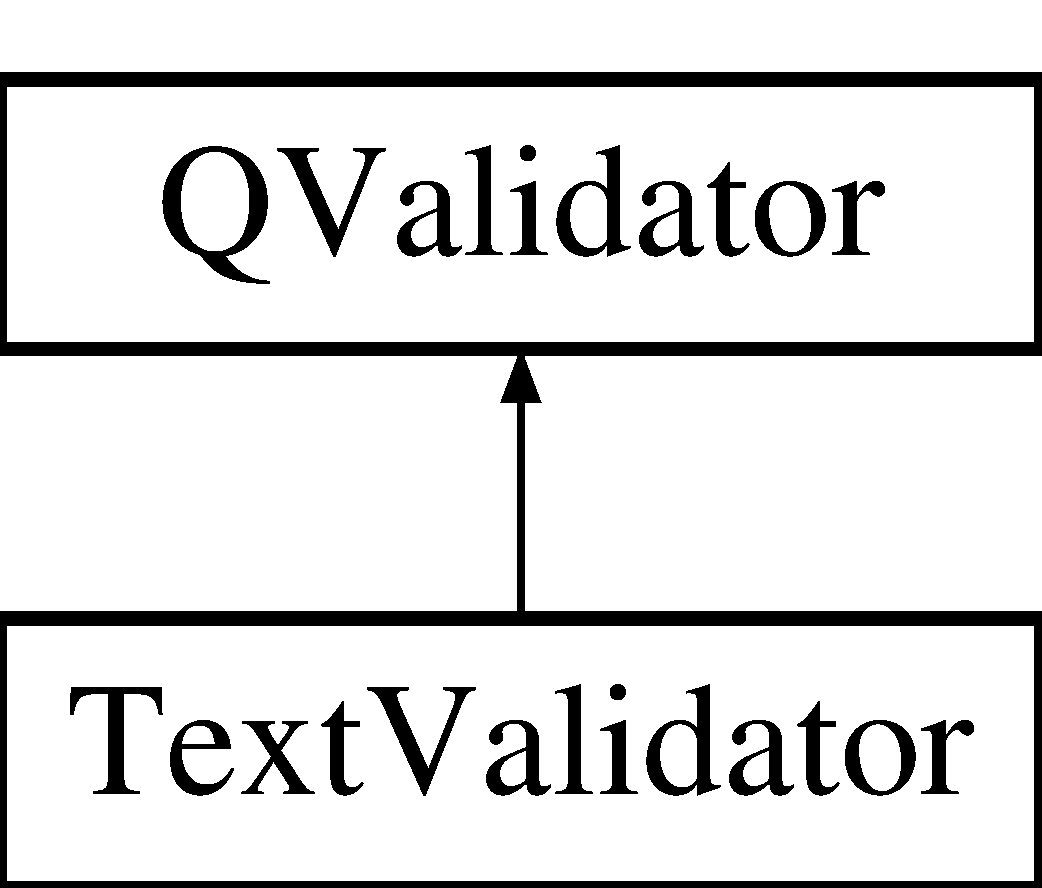
\includegraphics[height=2.000000cm]{class_text_validator}
\end{center}
\end{figure}
\subsection*{Открытые члены}
\begin{DoxyCompactItemize}
\item 
\hyperlink{class_text_validator_a29a44f791c6a0236b562f847deefa527}{Text\+Validator} (Q\+Object $\ast$parent=0)
\begin{DoxyCompactList}\small\item\em \hyperlink{class_text_validator_a29a44f791c6a0236b562f847deefa527}{Text\+Validator\+::\+Text\+Validator}. \end{DoxyCompactList}\item 
State \hyperlink{class_text_validator_a42a94c8bf5655196978addd3a2124582}{validate} (Q\+String \&, int \&) const 
\begin{DoxyCompactList}\small\item\em \hyperlink{class_text_validator_a42a94c8bf5655196978addd3a2124582}{Text\+Validator\+::validate}. \end{DoxyCompactList}\end{DoxyCompactItemize}


\subsection{Конструктор(ы)}
\index{Text\+Validator@{Text\+Validator}!Text\+Validator@{Text\+Validator}}
\index{Text\+Validator@{Text\+Validator}!Text\+Validator@{Text\+Validator}}
\subsubsection[{\texorpdfstring{Text\+Validator(\+Q\+Object $\ast$parent=0)}{TextValidator(QObject *parent=0)}}]{\setlength{\rightskip}{0pt plus 5cm}Text\+Validator\+::\+Text\+Validator (
\begin{DoxyParamCaption}
\item[{Q\+Object $\ast$}]{parent = {\ttfamily 0}}
\end{DoxyParamCaption}
)}\hypertarget{class_text_validator_a29a44f791c6a0236b562f847deefa527}{}\label{class_text_validator_a29a44f791c6a0236b562f847deefa527}


\hyperlink{class_text_validator_a29a44f791c6a0236b562f847deefa527}{Text\+Validator\+::\+Text\+Validator}. 


\begin{DoxyParams}{Аргументы}
{\em parent} & \\
\hline
\end{DoxyParams}


\subsection{Методы}
\index{Text\+Validator@{Text\+Validator}!validate@{validate}}
\index{validate@{validate}!Text\+Validator@{Text\+Validator}}
\subsubsection[{\texorpdfstring{validate(\+Q\+String \&, int \&) const }{validate(QString &, int &) const }}]{\setlength{\rightskip}{0pt plus 5cm}Q\+Validator\+::\+State Text\+Validator\+::validate (
\begin{DoxyParamCaption}
\item[{Q\+String \&}]{text, }
\item[{int \&}]{pos}
\end{DoxyParamCaption}
) const}\hypertarget{class_text_validator_a42a94c8bf5655196978addd3a2124582}{}\label{class_text_validator_a42a94c8bf5655196978addd3a2124582}


\hyperlink{class_text_validator_a42a94c8bf5655196978addd3a2124582}{Text\+Validator\+::validate}. 


\begin{DoxyParams}{Аргументы}
{\em text} & \\
\hline
{\em pos} & \\
\hline
\end{DoxyParams}
\begin{DoxyReturn}{Возвращает}

\end{DoxyReturn}


Объявления и описания членов классов находятся в файлах\+:\begin{DoxyCompactItemize}
\item 
customvalidator.\+h\item 
customvalidator.\+cpp\end{DoxyCompactItemize}

\hypertarget{class_word_validator}{}\section{Класс Word\+Validator}
\label{class_word_validator}\index{Word\+Validator@{Word\+Validator}}
Граф наследования\+:Word\+Validator\+:\begin{figure}[H]
\begin{center}
\leavevmode
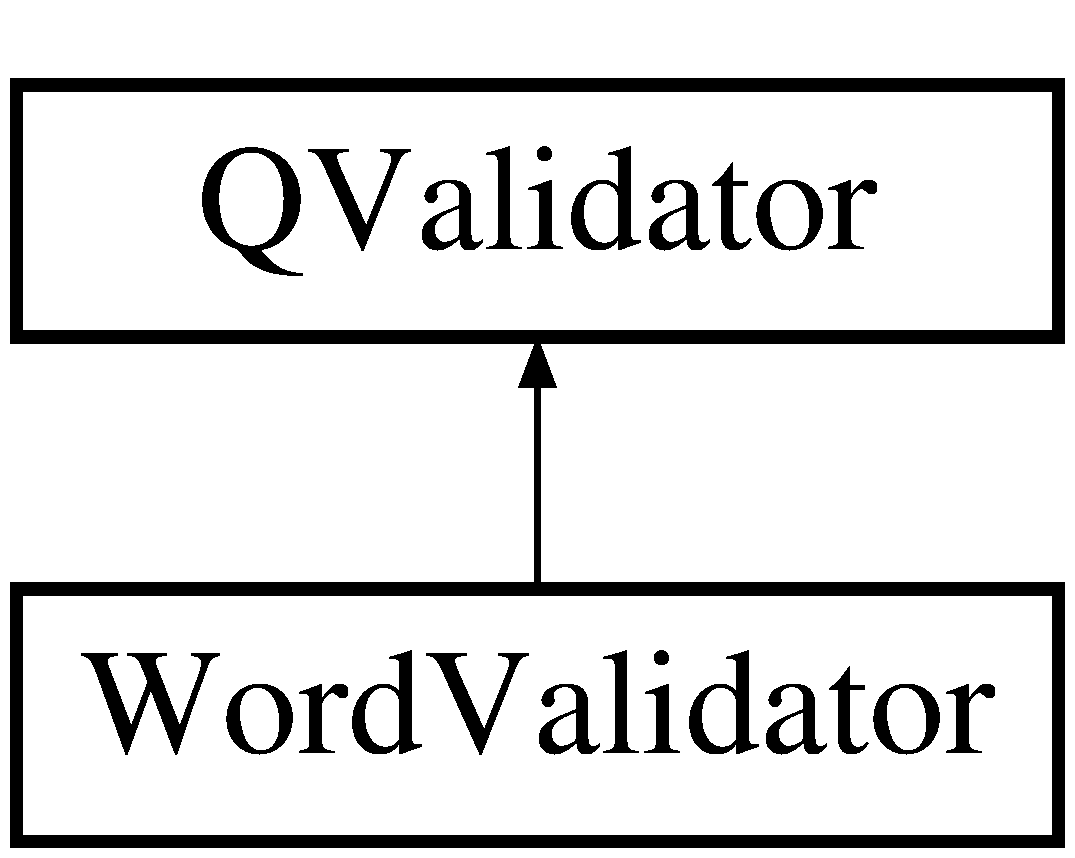
\includegraphics[height=2.000000cm]{class_word_validator}
\end{center}
\end{figure}
\subsection*{Открытые члены}
\begin{DoxyCompactItemize}
\item 
\hyperlink{class_word_validator_a055e67ae8b4af520d431d6e2fadea006}{Word\+Validator} (Q\+Object $\ast$parent=0)
\begin{DoxyCompactList}\small\item\em \hyperlink{class_word_validator_a055e67ae8b4af520d431d6e2fadea006}{Word\+Validator\+::\+Word\+Validator}. \end{DoxyCompactList}\item 
State \hyperlink{class_word_validator_afa4709ee674801c25513b588c8a3d0c1}{validate} (Q\+String \&, int \&) const 
\begin{DoxyCompactList}\small\item\em \hyperlink{class_word_validator_afa4709ee674801c25513b588c8a3d0c1}{Word\+Validator\+::validate}. \end{DoxyCompactList}\end{DoxyCompactItemize}


\subsection{Конструктор(ы)}
\index{Word\+Validator@{Word\+Validator}!Word\+Validator@{Word\+Validator}}
\index{Word\+Validator@{Word\+Validator}!Word\+Validator@{Word\+Validator}}
\subsubsection[{\texorpdfstring{Word\+Validator(\+Q\+Object $\ast$parent=0)}{WordValidator(QObject *parent=0)}}]{\setlength{\rightskip}{0pt plus 5cm}Word\+Validator\+::\+Word\+Validator (
\begin{DoxyParamCaption}
\item[{Q\+Object $\ast$}]{parent = {\ttfamily 0}}
\end{DoxyParamCaption}
)}\hypertarget{class_word_validator_a055e67ae8b4af520d431d6e2fadea006}{}\label{class_word_validator_a055e67ae8b4af520d431d6e2fadea006}


\hyperlink{class_word_validator_a055e67ae8b4af520d431d6e2fadea006}{Word\+Validator\+::\+Word\+Validator}. 


\begin{DoxyParams}{Аргументы}
{\em parent} & \\
\hline
\end{DoxyParams}


\subsection{Методы}
\index{Word\+Validator@{Word\+Validator}!validate@{validate}}
\index{validate@{validate}!Word\+Validator@{Word\+Validator}}
\subsubsection[{\texorpdfstring{validate(\+Q\+String \&, int \&) const }{validate(QString &, int &) const }}]{\setlength{\rightskip}{0pt plus 5cm}Q\+Validator\+::\+State Word\+Validator\+::validate (
\begin{DoxyParamCaption}
\item[{Q\+String \&}]{text, }
\item[{int \&}]{pos}
\end{DoxyParamCaption}
) const}\hypertarget{class_word_validator_afa4709ee674801c25513b588c8a3d0c1}{}\label{class_word_validator_afa4709ee674801c25513b588c8a3d0c1}


\hyperlink{class_word_validator_afa4709ee674801c25513b588c8a3d0c1}{Word\+Validator\+::validate}. 


\begin{DoxyParams}{Аргументы}
{\em text} & \\
\hline
{\em pos} & \\
\hline
\end{DoxyParams}
\begin{DoxyReturn}{Возвращает}

\end{DoxyReturn}


Объявления и описания членов классов находятся в файлах\+:\begin{DoxyCompactItemize}
\item 
customvalidator.\+h\item 
customvalidator.\+cpp\end{DoxyCompactItemize}

%--- End generated contents ---

% Index
\backmatter
\newpage
\phantomsection
\clearemptydoublepage
\addcontentsline{toc}{chapter}{Алфавитный указатель}
\printindex

\end{document}
